%%%%%%%%%%%%%%%%%%%%%%%%%%%%%%%%%%%%%%%%%
% A beamer poster style for the University of Oxford. Atilim Gunes Baydin <gunes@robots.ox.ac.uk>, November 2016.
% Based on the I6pd2 style created by Thomas Deselaers an Philippe Dreuw.
%
% Dreuw & Deselaer's Poster
% LaTeX Template
% Version 1.0 (11/04/13)
%
% Created by:
% Philippe Dreuw and Thomas Deselaers
% http://www-i6.informatik.rwth-aachen.de/~dreuw/latexbeamerposter.php
%
% This template has been downloaded from:
% http://www.LaTeXTemplates.com
%
% License:
% CC BY-NC-SA 3.0 (http://creativecommons.org/licenses/by-nc-sa/3.0/)
%
%%%%%%%%%%%%%%%%%%%%%%%%%%%%%%%%%%%%%%%%%

%----------------------------------------------------------------------------------------
%   PACKAGES AND OTHER DOCUMENT CONFIGURATIONS
%----------------------------------------------------------------------------------------

\documentclass[final,hyperref={pdfpagelabels=false}]{beamer}

\usepackage[orientation=portrait,size=a0,scale=1.3]{beamerposter} % Use the beamerposter package for laying out the poster with a portrait orientation and an a0 paper size

\usetheme{Demo}

\usepackage[utf8]{inputenc} % allow utf-8 input
\usepackage{blindtext}
\usepackage{amsmath,amsthm,amssymb,latexsym} % For including math equations, theorems, symbols, etc
\usepackage[document]{ragged2e}
%\usepackage{times}\usefonttheme{professionalfonts}  % Uncomment to use Times as the main font
\usefonttheme[onlymath]{serif} % Uncomment to use a Serif font within math environments
%\boldmath % Use bold for everything within the math environment
\usepackage{booktabs} % Top and bottom rules for tables
\usepackage{microtype}

\usepackage{graphicx}
\usepackage{listings}
\usepackage{float}
\usepackage{natbib}
\bibliographystyle{plainnat}

\usecaptiontemplate{\small\structure{\insertcaptionname~\insertcaptionnumber: }\insertcaption} % A fix for figure numbering

\newcommand{\shrink}{-15pt}

\def\imagetop#1{\vtop{\null\hbox{#1}}}

\let\oldbibliography\thebibliography
\renewcommand{\thebibliography}[1]{\oldbibliography{#1}
	\setlength{\itemsep}{-10pt}}

%----------------------------------------------------------------------------------------
%   TITLE SECTION 
%----------------------------------------------------------------------------------------
\title{\Huge Modelling Population Riots} % Poster title
\author{Angus Blance}
\institute{University of Dundee}

%----------------------------------------------------------------------------------------
%   FOOTER TEXT
%----------------------------------------------------------------------------------------
\newcommand{\leftfoot}{} % Left footer text
\newcommand{\rightfoot}{} % Right footer text


%----------------------------------------------------------------------------------------

\begin{document}
	\addtobeamertemplate{block end}{}{\vspace*{2ex}} % White space under blocks
	
	\begin{frame}[t] % The whole poster is enclosed in one beamer frame
		
		\begin{columns}[t] % The whole poster consists of three major columns, each of which can be subdivided further with another \begin{columns} block - the [t] argument aligns each column's content to the top
				
				\begin{column}{.03\textwidth}\end{column} % Empty spacer column
				
				%%%%%%%%%%%%%%%%%%%%%%%%%%%%%%%%%%%%%%%%%%
				%% Column 1
				%%%%%%%%%%%%%%%%%%%%%%%%%%%%%%%%%%%%%%%%%%
				
				\begin{column}{.32\textwidth} % 1st column
					
					\vspace{\shrink}          
					\begin{block}{Abstract}
						Using Epstein's Agent Based Civil Violence Model To suppress Rebellion, as swell as see how smoke can be used to suppress an uprising. 
					\end{block}
					
					\begin{block}{Introduction}
						Instances of large-scale disorder occur frequently around the world,
						resulting in significant damage to property and, at times, human
						life. Given the destructive nature of such events, it is crucial to
						develop models that can accurately capture the dynamics of rioting and identify potential strategies for mitigating the damage. In
						this report, we present an agent-based model (ABM) that replicates the behaviour of riot populations, and we demonstrate how
						the use of smoke by police forces can effectively reduce the number
						of participants in a riot.
					\end{block}
				
					\begin{block}{Mathematical Model}
						
						First off every agent has a certain level of risk aversion (R), the amount an individual will avoid risk, and a level of Hardship (H). As well as vision (v) which is an area around each individual in which they scan and count the number of people around them. \\
						
						The grievance (G) that someone has is given by: 
						\begin{equation}
							G = H(L-1)
						\end{equation}
						
						
						Probability of a non police officer agent to get arrested is given by:
						\begin{equation}
							P = 1 - EXP(-k(C/A)_{v})
						\end{equation}
						 where C the number of police in v and A the number of active's in v. k is determined by if C=A=1 then we have P=0.9 hence we have k=-ln(0.1)
						
						With R and P now defined we can calculate the net Risk N = RP giving us our final rule
					
						we now  have all we need to create the agent rule:\\
						\begin{equation}
							Agent \; rule: if \; G-N>T \; riot; \; otherwise \; stay \; a \;  civilian
						\end{equation}
						so the difference in G and N is the expected utility of expressing ones private grievance whilst T is the utility of not.
						
						
					\end{block}
				\begin{block}{Reduction in Police Forces}
					
				\begin{figure}[H]
					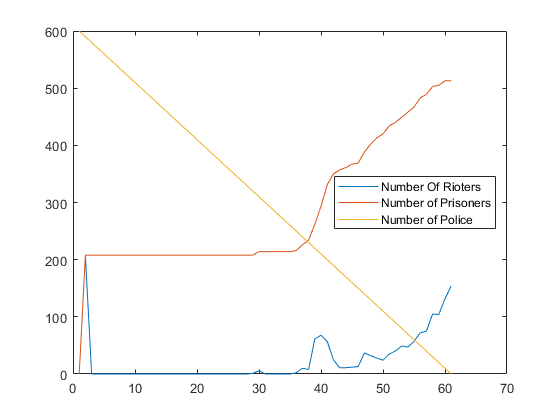
\includegraphics[width=\linewidth]{Police Reductions.png}
					\caption{C=600,Q=800,v=2,L=0.4,T=0.1}
					\label{fig:frenchriot}
				\end{figure}
			\end{block}
				\begin{block}{Conclusions}
					\begin{itemize}
						\item A sudden drop in Perceived Legitimacy of a government can cause an uprising
						\item Obscuring vision can help prevent large scale disorder
						\item Outrage towards a government has a "snowball" like affect
					\end{itemize}
			\end{block}
		\begin{block}{References}
			1. Epstein, Joshua M. Modeling civil violence: An agent-based computational approach. 2002\\
		2. Bonnasse-Gahot, Laurent and Berestycki, Henri and Depuiset, Marie-Aude and Gordon, Mirta B and Roch{\'e}, Sebastian and Rodriguez, Nancy and Nadal, Jean-Pierre. Epidemiological modelling of the 2005 French riots: a spreading wave and the role of contagion. 2018
	
	\end{block}
		
		
					
				\end{column} % End of the 1st column
				
				%%%%%%%%%%%%%%%%%%%%%%%%%%%%%%%%%%%%%%%%%%
				%% Column 2
				%%%%%%%%%%%%%%%%%%%%%%%%%%%%%%%%%%%%%%%%%%
				
				\begin{column}{.02\textwidth}\end{column} % Empty spacer column
				
				\begin{column}{.32\textwidth} % 2nd column
					\vspace{\shrink}
					\begin{block}{Computational Model}
						
				
					
					-Agent Movement
					\begin{figure}[H]
						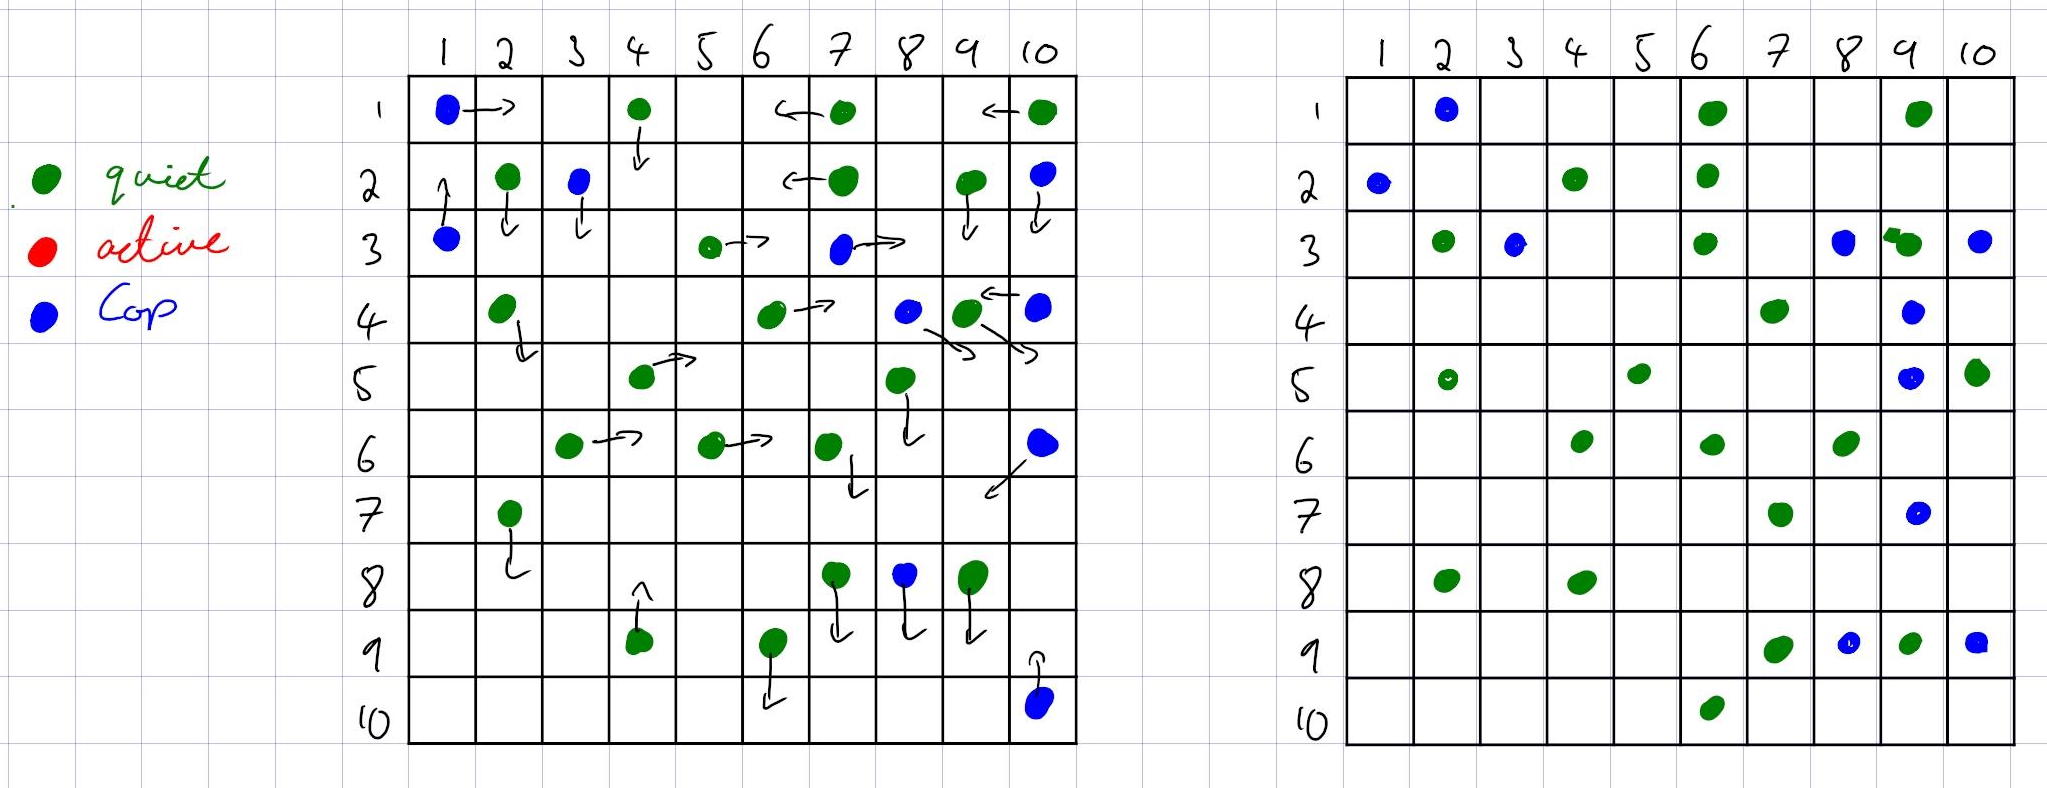
\includegraphics[width=\linewidth]{Movement visual.png}
						\caption{Agent Movement}
						\label{fig:frenchriot}
					\end{figure}
					
					-Vision
					\begin{figure}[H]
						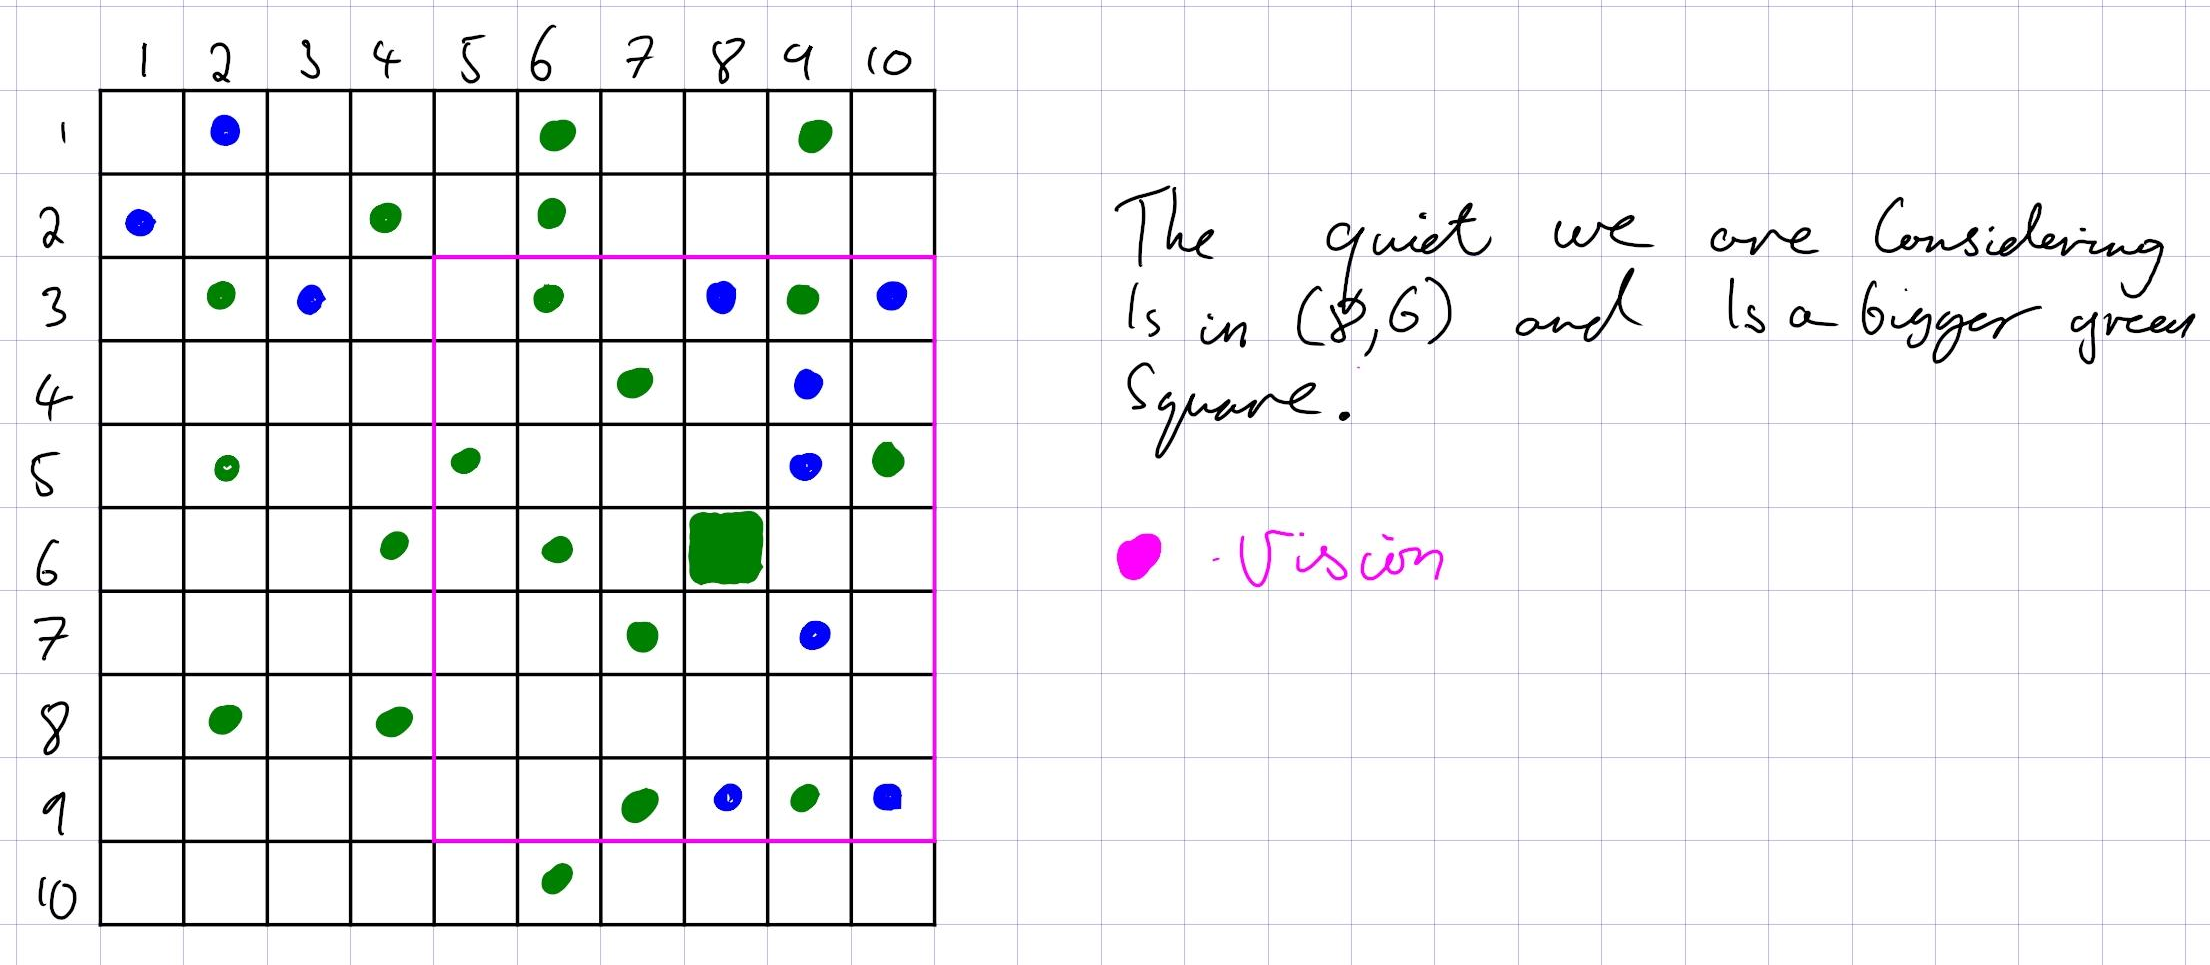
\includegraphics[width=\linewidth]{vision for single case.png}
						\caption{Vision}
						\label{fig:frenchriot}
					\end{figure}	
					
					-Arresting
					\begin{figure}[H]
						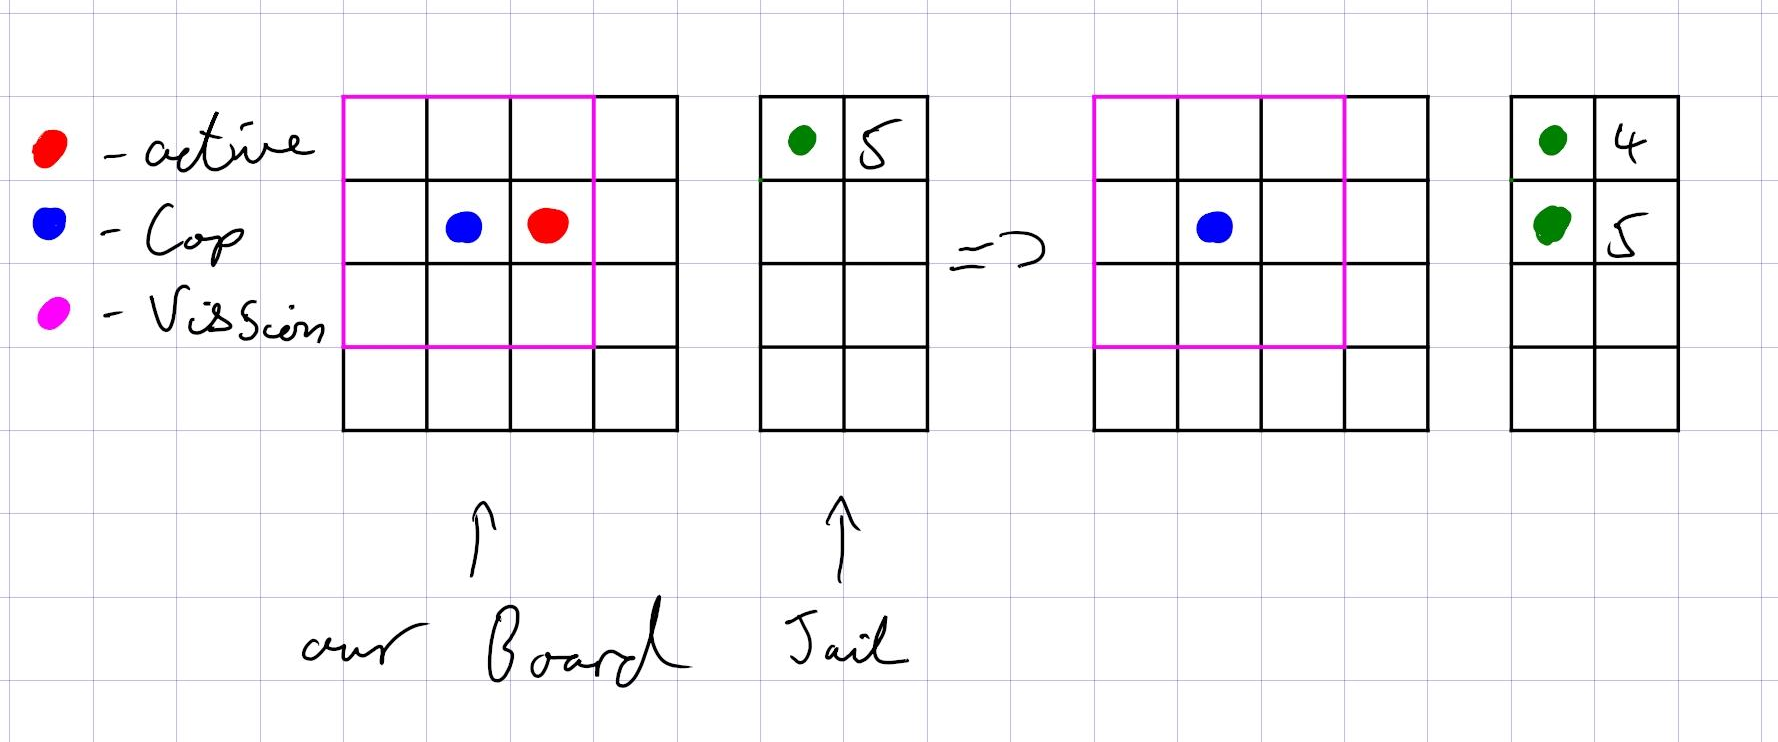
\includegraphics[width=\linewidth]{arresting visual.png}
						\caption{Arresting}
						\label{fig:frenchriot}
					\end{figure}	
					-Smoke
					\begin{figure}[H]
						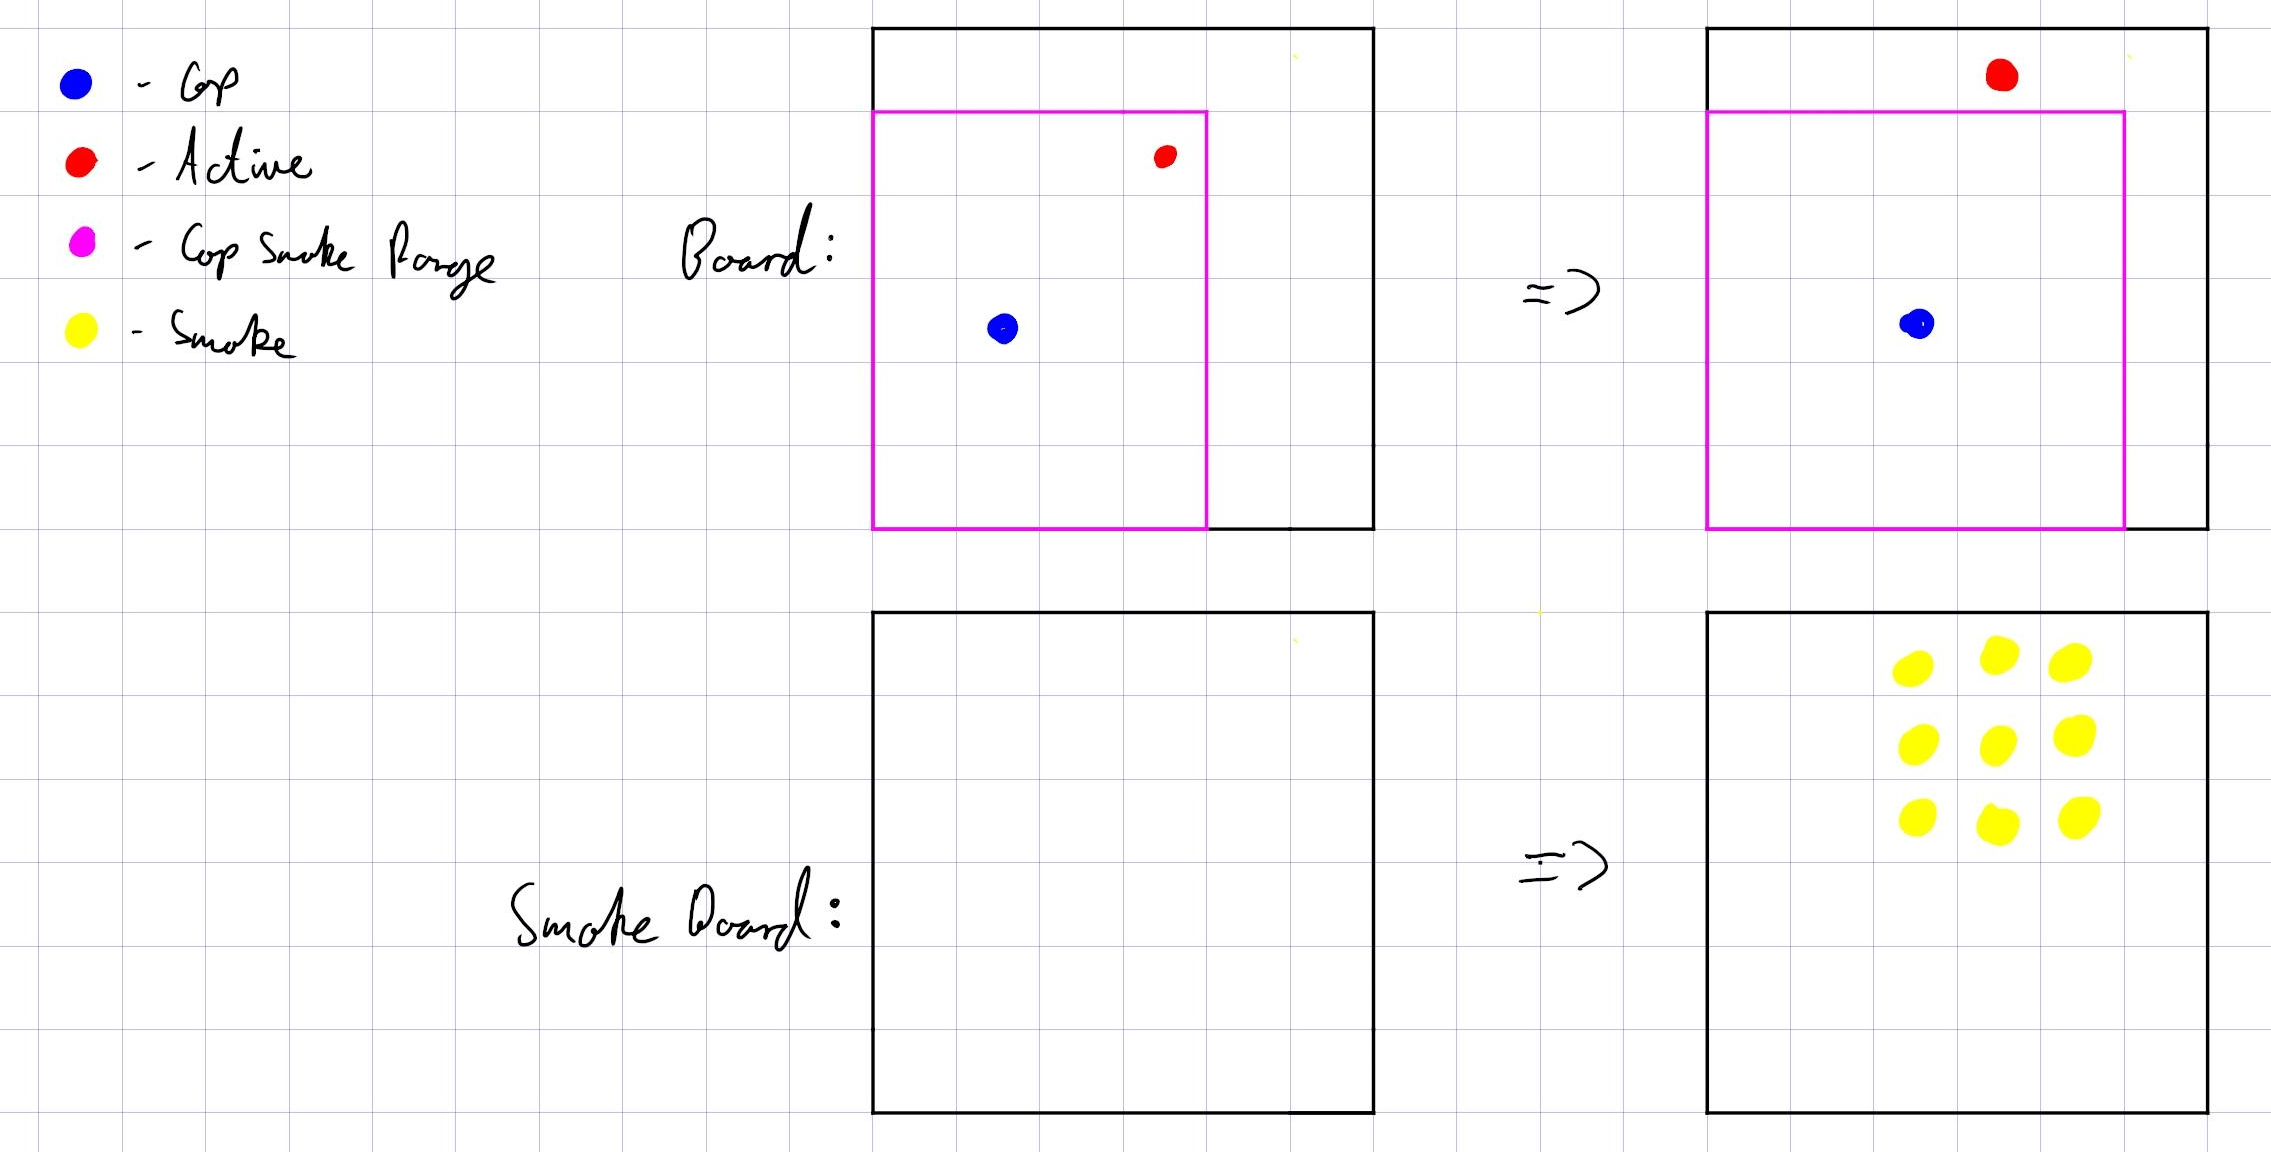
\includegraphics[width=\linewidth]{smoke visual.png}
						\caption{Police Smoke}
						\label{fig:frenchriot}
					\end{figure}	
					
					\end{block}
				\begin{block}{Agent Behaviour}
					-Deceptive Behaviour\\
					-Snowball Effect
					\begin{figure}[H]
						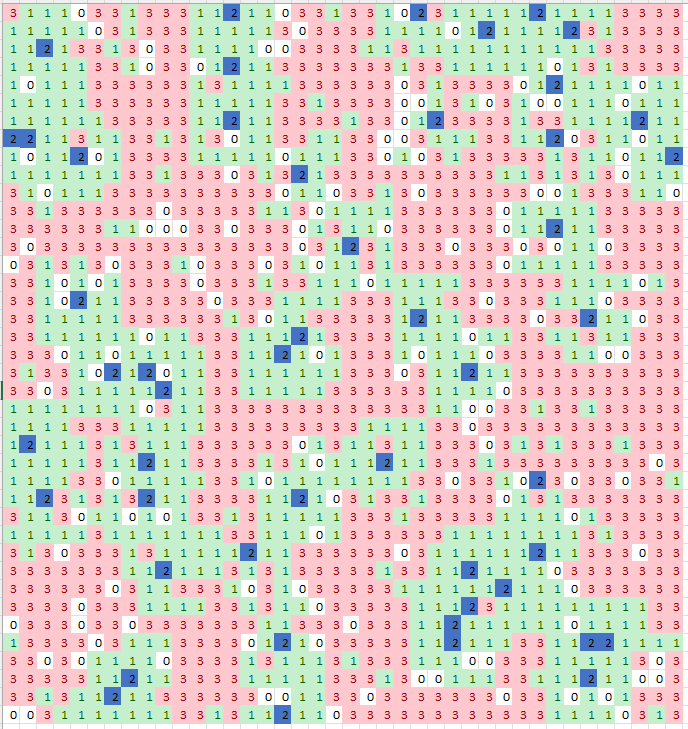
\includegraphics[width=\linewidth]{snowball_2.png}
						\caption{C=1400,Q=50,V=2,T = 0.01, L=0.89}
						\label{fig:}
					\end{figure}
					
				
			
				\end{block}
					
				
					
				\end{column} % End of the 2nd column
				
				%%%%%%%%%%%%%%%%%%%%%%%%%%%%%%%%%%%%%%%%%%
				%% Column 3
				%%%%%%%%%%%%%%%%%%%%%%%%%%%%%%%%%%%%%%%%%%
				
				
				
				
				\begin{column}{.02\textwidth}\end{column} % Empty spacer column
				\begin{column}{.3\textwidth} % 2nd column
					\begin{block}{Effect of legitimacy}
					Slow Decline of Legitimacy
				
					\begin{figure}[H]
						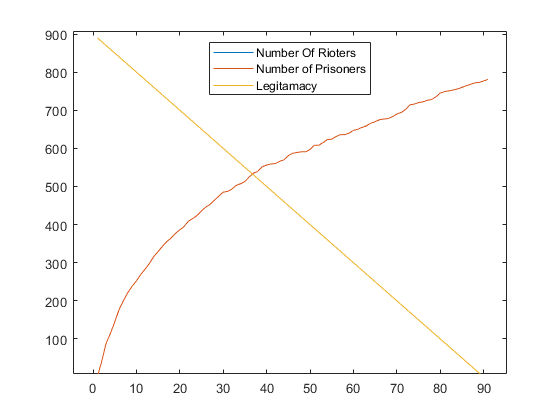
\includegraphics[width=\linewidth]{effect of Legitamacy reduction.png}
						\caption{C=50,Q=1400,v=2,T=0.1,L=0.9-0}
						\label{fig:yu}
					\end{figure}
					Sudden Drop In Legitimacy
					\begin{figure}[H]
					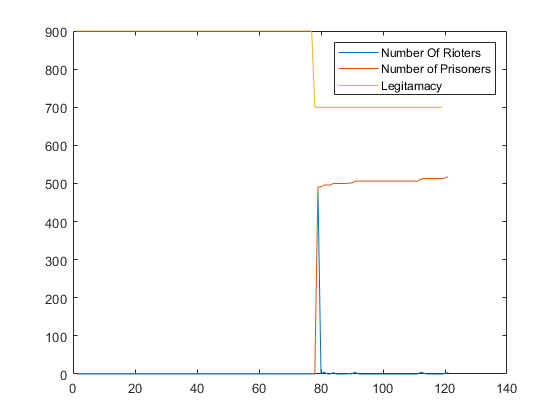
\includegraphics[width=\linewidth]{sudden effect of Legitamacy reduction.png}
					\caption{C=50,Q=1400,v=2,T=0.1,L=0.9,0.7}
					\label{fig:frenchriot}
				\end{figure}
					\end{block}
			\begin{block}{periodic Outbursts Of Violence}
					-Periodic Outbursts of Violence
					\begin{figure}[H]
						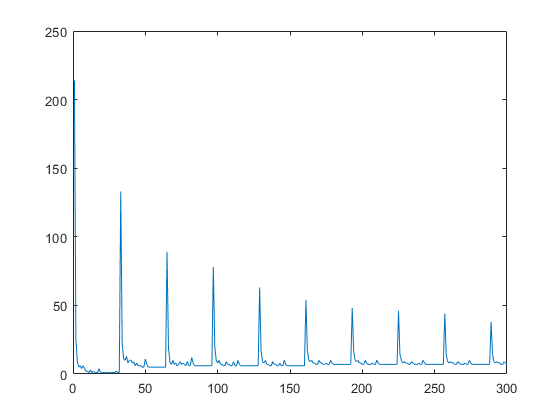
\includegraphics[width=\linewidth]{Outbursts_of_violence.png}
						\caption{C=50,Q=1400,v=2,T=0.1,L=0.89}
						\label{fig:yu}
					\end{figure}
					-Smoke Used To Reduce Number Of Actives
					\begin{figure}[H]
						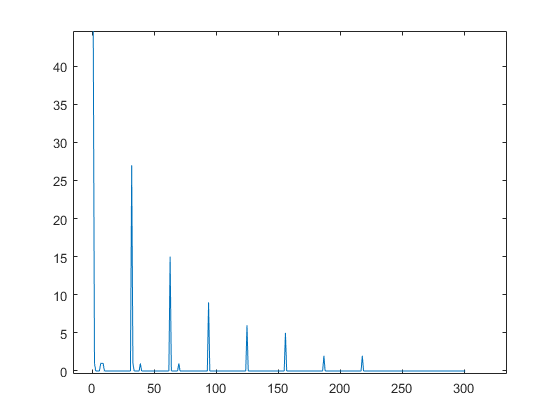
\includegraphics[width=\linewidth]{Smokes_affect_on_Outbursts.png}
						\caption{C=50,Q=1400,v=2,T=0.1,L=0.89}
						\label{fig:yu}
					\end{figure}
			\end{block}
					
				\end{column}
					
			\end{columns} % End of all the columns in the poster
		\end{frame} % End of the enclosing frame
		
	\end{document}